\ylDisplay
{}% Problem name
{2021}% Year
{mcq}% Round (mcq, theory, experiment)
{9}% Problem nr.
{physics}% Subject (physics, chemistry, biology)
{}% Difficulty (1-3)
{
% Syl:
\ifStatement
A typical ping pong ball is dropped from a height of 1 m above a marble floor. The ball bounces several times before it comes to rest. For every successive bounce, it loses \SI{20}{\percent} of its maximum height. Fatima plotted two quantities that she observed in this phenomenon and the graphs are shown below. Identify the two quantities plotted on the vertical axis. (Air resistance is neglected.)
\begin{center}
  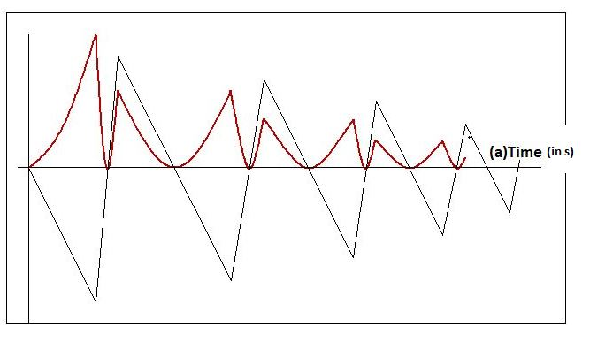
\includegraphics[width=0.7\linewidth]{2021-mcq-09-p}
\end{center}
\fi


\ifOption1
Height and velocity
\fi


\ifOption2
Velocity and kinetic energy
\fi


\ifOption3
Potential energy and kinetic energy
\fi


\ifOption4
Velocity and potential energy
\fi


\ifHint

\fi


\ifSolution

\fi


\ifEstStatement
% Problem name:

\fi


\ifEstOption1

\fi


\ifEstOption2

\fi


\ifEstOption3

\fi


\ifEstOption4

\fi


\ifEstHint

\fi


\ifEstSolution

\fi
}
